\documentclass[../PianoDiProgetto.tex]{subfiles}
\begin{document}
	\section{Preventivo}
		\subsection{Analisi}
			\subsubsection{Prospetto orario}
			\begin{table}[H]
			\center
				\begin{tabular}{cccccccc}
				\noalign{\hrule height 1.5pt}
				\textbf{Nome} & \textbf{Res} & \textbf{Amm} & \textbf{An} & \textbf{Pt} & \textbf{Pr} & \textbf{Ve} & \textbf{Totale} \\ \hline
				Bonato Enrico & - & - & 5 & - & - & 5 & 10 \\ \hline
				Bonolo Marco  & - & - & 8 & - & - & - & 8 \\ \hline
				Pace Giulio  & - & 5 & 8 & - & - & 6 & 19 \\ \hline
				Pezzuto Francesco  & 2 & - & 9 & - & - & 8 & 19 \\ \hline
				Sanna Giovanni  & 2 & 4 & 7 & - & - & 5 & 18 \\ \hline
				Sovilla Matteo  & 8 & - & 7 & - & - & - & 15  \\ \hline
				\textbf{Ore Totali Ruolo} & \textbf{12} & \textbf{9} & \textbf{44} & \textbf{0} & \textbf{0} & \textbf{24} & \textbf{89} \\ \hline
				\noalign{\hrule height 1.5pt}
				\end{tabular}
			\caption{Prospetto orario Analisi.  \label{tab:table_label}}
			\end{table}
			\begin{figure}[H]
				\centering
				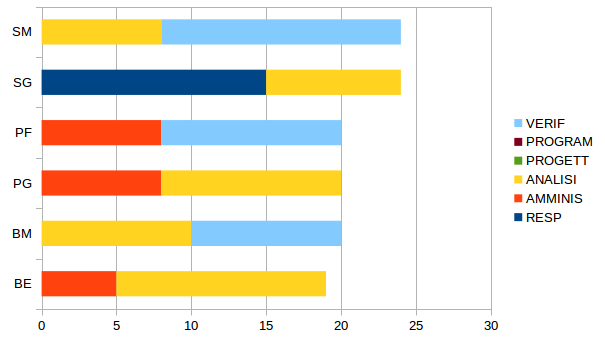
\includegraphics[scale=0.7]{Figures/OreComponenteAnalisi.png}
				\caption{Analisi: ore per componente.}\label{fig:1}
			\end{figure}
			\begin{figure}[H]
				\centering
				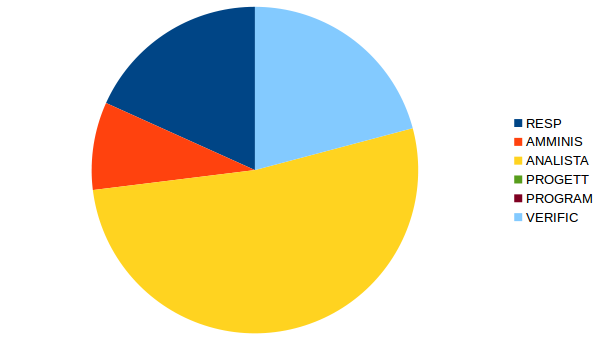
\includegraphics[scale=0.7]{Figures/OreRuoloAnalisi.png}
				\caption{Analisi: ore per ruolo.}\label{fig:2}
			\end{figure}
			
			\subsubsection{Prospetto economico}
			\begin{table}[H]
				\center
				\begin{tabular}{|c|c|c|}
					\noalign{\hrule height 1.5pt}
					\textbf{Ruolo} & \textbf{Ore} & \textbf{Costo(\euro)}     \\
					\hline
					Responsabile  & 12 & 360\\ 
					\hline
					Amministratore  & 9  & 180\\
					\hline
					Analista  & 44 & 1100\\
					\hline
					Progettista  & 0 & 0\\
					\hline
					Programmatore  & 0 & 0\\
					\hline
					Verificatore  & 24 & 360\\
					\hline
					\textbf{Totale}  & \textbf{89} & \textbf{2000}\\
					\noalign{\hrule height 1.5pt}
			\end{tabular}
			\caption{Prospetto economico Analisi.  \label{tab:table_label}}
		\end{table}
		
		\subsection{Analisi di dettaglio}
			\subsubsection{Prospetto orario} 
			\begin{table}[H]
			\center
				\begin{tabular}{cccccccc}
				\noalign{\hrule height 1.5pt}
				\textbf{Nome} & \textbf{Res} & \textbf{Amm} & \textbf{An} & \textbf{Pt} & \textbf{Pr} & \textbf{Ve} & \textbf{Totale} \\ \hline
				Bonato Enrico & - & - & - & - & - & 12 & 12 \\ \hline
				Bonolo Marco  & - & - & 10 & - & - & - & 10 \\ \hline
				Pace Giulio  & - & - & - & - & - & 12 & 12 \\ \hline
				Pezzuto Francesco  & - & - & 12 & - & - & - & 12 \\ \hline
				Sanna Giovanni  & - & - & 17 & - & - & - & 17 \\ \hline
				Sovilla Matteo  & 5 & 5 & - & - & - & 5 & 15 \\ \hline
				\textbf{Ore Totali Ruolo} & \textbf{5} & \textbf{5} & \textbf{39} & \textbf{0} & \textbf{0} & \textbf{29} & \textbf{78} \\ \hline
				\noalign{\hrule height 1.5pt}
				\end{tabular}
			\caption{Prospetto orario Analisi di dettaglio.  \label{tab:table_label}}
			\end{table}
			\begin{figure}[H]
				\centering
				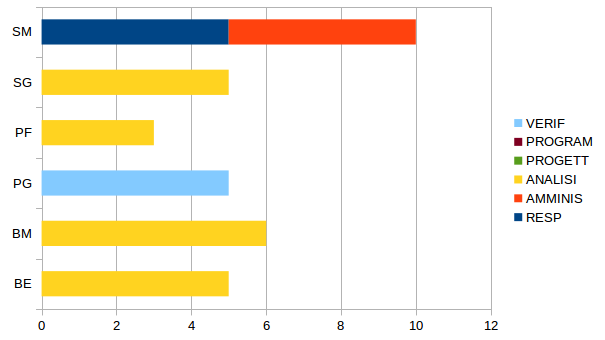
\includegraphics[scale=0.7]{Figures/OreComponenteAnalisiDett.png}
				\caption{Analisi di dettaglio: ore per componente.}\label{fig:4}
			\end{figure}
			\begin{figure}[H]
				\centering
				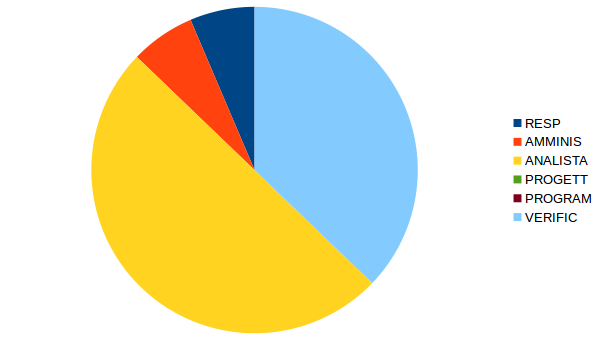
\includegraphics[scale=0.7]{Figures/OreRuoloAnalisiDett.png}
				\caption{Analisi di dettaglio: ore per ruolo.}\label{fig:5}
		\end{figure}
			
			\subsubsection{Prospetto economico}
			\begin{table}[H]
				\center
				\begin{tabular}{|c|c|c|}
					\noalign{\hrule height 1.5pt}
					\textbf{Ruolo} & \textbf{Ore} & \textbf{Costo(\euro)}     \\
					\hline
					Responsabile  & 5 & 150 \\
					\hline
					Amministratore  & 5  & 100 \\
					\hline
					Analista  & 39  & 975\\
					\hline
					Progettista  & 0 & 0\\
					\hline
					Programmatore  & 0 & 0\\
					\hline
					Verificatore  & 29 & 435\\
					\hline
					\textbf{Totale}  & \textbf{78} & \textbf{1560}\\
					\noalign{\hrule height 1.5pt}
			\end{tabular}
			\caption{Prospetto economico Analisi di dettaglio.  \label{tab:table_label}}
		\end{table}
		
		
		\subsection{Progettazione architetturale}
			\subsubsection{Prospetto orario}
			\begin{table}[H]
			\center
				\begin{tabular}{cccccccc}
				\noalign{\hrule height 1.5pt}
				\textbf{Nome} & \textbf{Res} & \textbf{Amm} & \textbf{An} & \textbf{Pt} & \textbf{Pr} & \textbf{Ve} & \textbf{Totale} \\ \hline
				Bonato Enrico & 6 & - & 14 & 12 & - & - & 32 \\ \hline
				Bonolo Marco  & - & 8 & - & 14 & - & 24 & 32 \\ \hline
				Pace Giulio  & 6 & - & 10 & 10 & - & - & 26 \\ \hline
				Pezzuto Francesco  & - & - & 12 & 13 & - & - & 25 \\ \hline
				Sanna Giovanni  & - & 10 & - & - & - & 16 & 26 \\ \hline
				Sovilla Matteo  & - & - & 18 & 14 & - & - & 32 \\ \hline
				\textbf{Ore Totali Ruolo} & \textbf{12} & \textbf{18} & \textbf{55} & \textbf{48} &  \textbf{0}& \textbf{40} & \textbf{173} \\ \hline
				\noalign{\hrule height 1.5pt}
				\end{tabular}
			\caption{Prospetto orario Progettazione architetturale.  \label{tab:table_label}}
			\end{table}
			\begin{figure}[H]
				\centering
				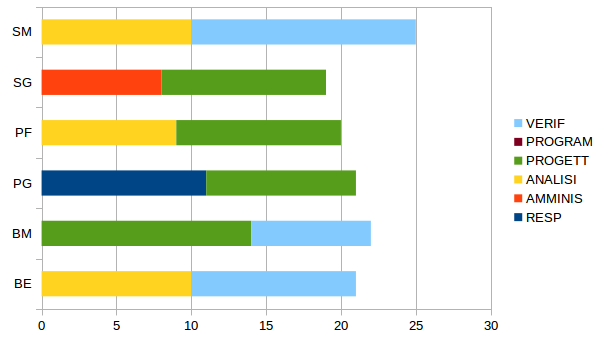
\includegraphics[scale=0.7]{Figures/OreComponenteProgArch.png}
				\caption{Progettazione architetturale: ore per componente.}\label{fig:7}
			\end{figure}
			\begin{figure}[H]
				\centering
				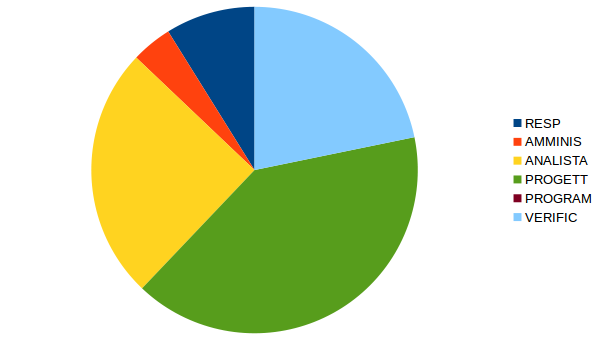
\includegraphics[scale=0.7]{Figures/OreRuoloProgArch.png}
				\caption{Progettazione architetturale: ore per ruolo.}\label{fig:8}
			\end{figure}
			
			\subsubsection{Prospetto economico}
			\begin{table}[H]
				\center
				\begin{tabular}{|c|c|c|}
					\noalign{\hrule height 1.5pt}
					\textbf{Ruolo} & \textbf{Ore} & \textbf{Costo(\euro)}     \\
					\hline
					Responsabile  & 12 & 360 \\
					\hline
					Amministratore  &  18 & 360 \\
					\hline
					Analista  & 55 & 1375 \\
					\hline
					Progettista  & 48 & 1056 \\
					\hline
					Programmatore  & 0 & 0 \\
					\hline 
					Verificatore  & 40 & 600 \\
					\hline
					\textbf{Totale}  & \textbf{173} & \textbf{3751}\\
					\noalign{\hrule height 1.5pt}
			\end{tabular}
			\caption{Prospetto economico Progettazione architetturale.  \label{tab:table_label}}
		\end{table}
		
		
		\subsection{Progettazione di dettaglio e Codifica}
			\subsubsection{Prospetto orario}
			\begin{table}[H]
			\center
				\begin{tabular}{cccccccc}
				\noalign{\hrule height 1.5pt}
				\textbf{Nome} & \textbf{Res} & \textbf{Amm} & \textbf{An} & \textbf{Pt} & \textbf{Pr} & \textbf{Ve} & \textbf{Totale} \\ \hline
				Bonato Enrico & - & 12 & - & 21 & 15 & - & 48 \\ \hline
				Bonolo Marco  & 8 & - & -8 & - & 13 & 24 & 53 \\ \hline
				Pace Giulio  & - & - & - & 17 & 15 & 20 & 52 \\ \hline
				Pezzuto Francesco  & 4 & 5 & - & 16 & 12 & 16 & 53 \\ \hline
				Sanna Giovanni  & - & - & - & 16 & 12 & 21 & 49 \\ \hline
				Sovilla Matteo  & - & - & 6 & 22 & 14 & - & 42 \\ \hline
				\textbf{Ore Totali Ruolo} & \textbf{12} & \textbf{17} & \textbf{14} & \textbf{92} & \textbf{81} & \textbf{81} & \textbf{297} \\ \hline
				\noalign{\hrule height 1.5pt}
				\end{tabular}
			\caption{Prospetto orario Progettazione di dettaglio e Codifica.  \label{tab:table_label}}
			\end{table}
			\begin{figure}[H]
				\centering
				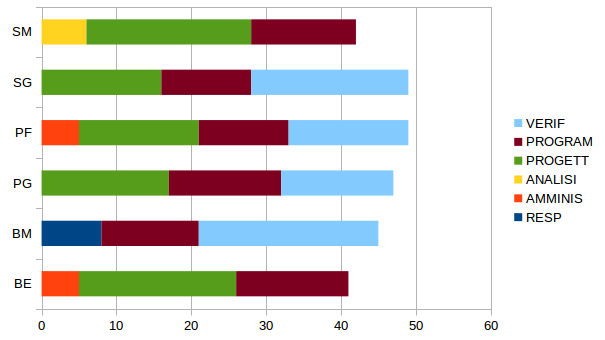
\includegraphics[scale=0.7]{Figures/OreComponenteProgDettCodifica.png}
				\caption{Progettazione di dettaglio e codifica: ore per componente.}\label{fig:10}
			\end{figure}
			\begin{figure}[H]
				\centering
				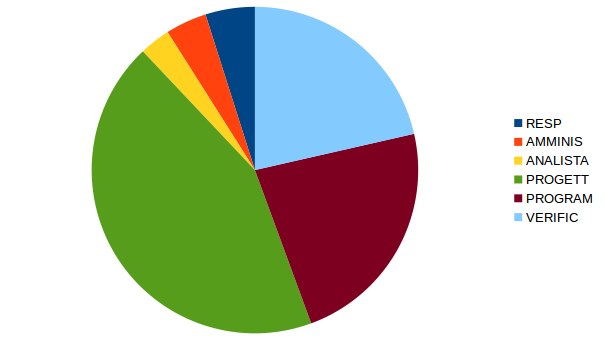
\includegraphics[scale=0.7]{Figures/OreRuoloProgDettCodifica.png}
				\caption{Progettazione di dettaglio e codifica: ore per ruolo.}\label{fig:11}
			\end{figure}
			
			\subsubsection{Prospetto economico}
			\begin{table}[H]
				\center
				\begin{tabular}{|c|c|c|}
					\noalign{\hrule height 1.5pt}
					\textbf{Ruolo} & \textbf{Ore} & \textbf{Costo(\euro)}     \\
					\hline
					Responsabile  & 12 & 360\\
					\hline
					Amministratore  & 17  & 340 \\
					\hline
					Analista  & 14  & 350 \\
					\hline
					Progettista  & 92 & 2024 \\
					\hline
					Programmatore  & 81 & 1215 \\
					\hline
					Verificatore  & 81 & 1215 \\
					\hline
					\textbf{Totale}  & \textbf{297} & \textbf{5504}\\
					\noalign{\hrule height 1.5pt}
			\end{tabular}
			\caption{Prospetto economico Progettazione di dettaglio e Codifica.  \label{tab:table_label}}
		\end{table}
		
		\subsection{Validazione}
			\subsubsection{Prospetto orario}
			\begin{table}[H]
			\center
				\begin{tabular}{cccccccc}
				\noalign{\hrule height 1.5pt}
				\textbf{Nome} & \textbf{Res} & \textbf{Amm} & \textbf{An} & \textbf{Pt} & \textbf{Pr} & \textbf{Ve} & \textbf{Totale} \\ \hline
				Bonato Enrico & - & - & - & 4 & 0 & 9 & 13 \\ \hline
				Bonolo Marco  & - & - & - & 4 & 6 & - & 10 \\ \hline
				Pace Giulio  & - & - & - & - & 6 & 9 & 15 \\ \hline
				Pezzuto Francesco  & - & 8 & - & - & - & 7 & 15 \\ \hline
				Sanna Giovanni  & 8 & - & - & - & 5 & - & 13 \\ \hline
				Sovilla Matteo  & - & - & - & - & - & 16 & 16 \\ \hline
				\textbf{Ore Totali Ruolo} & \textbf{8} & \textbf{8} & \textbf{0} & \textbf{8} 4969& \textbf{17} & \textbf{41} & \textbf{82} \\ \hline
				\noalign{\hrule height 1.5pt}
				\end{tabular}
			\caption{Prospetto orario Validazione.  \label{tab:table_label}}
			\end{table}
			\begin{figure}[H]
				\centering
				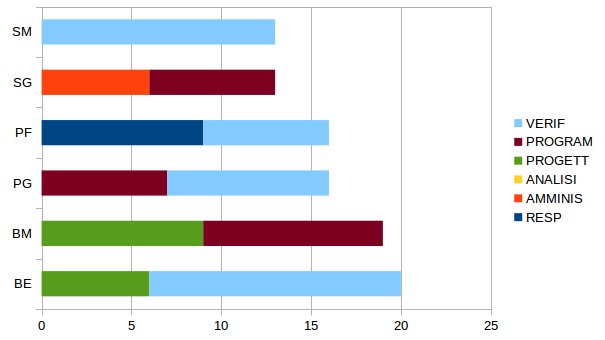
\includegraphics[scale=0.7]{Figures/OreComponenteValidazione.png}
				\caption{Validazione: ore per componente.}\label{fig:13}
			\end{figure}
			\begin{figure}[H]
				\centering
				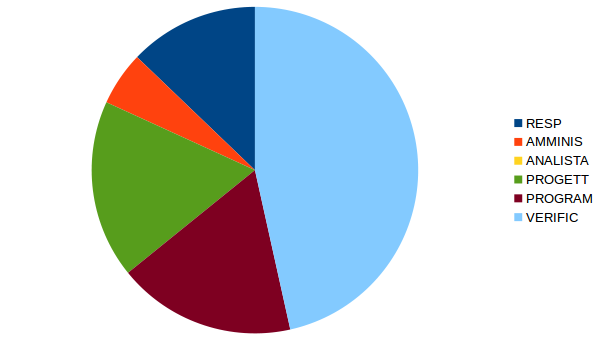
\includegraphics[scale=0.7]{Figures/OreRuoloValidazione.png}
				\caption{Validazione: ore per ruolo.}\label{fig:14}
			\end{figure}
			
			\subsubsection{Prospetto economico}
			\begin{table}[H]
				\center
				\begin{tabular}{|c|c|c|}
					\noalign{\hrule height 1.5pt}
					\textbf{Ruolo} & \textbf{Ore} & \textbf{Costo(\euro)}     \\
					\hline
					Responsabile  & 8 & 270 \\
					\hline
					Amministratore  & 8  & 160 \\
					\hline
					Analista  & 0  & 0 \\
					\hline
					Progettista  & 8 & 176 \\
					\hline
					Programmatore  & 17  & 255\\ 
					\hline
					Verificatore  & 41 & 615 \\
					\hline
					\textbf{Totale}  & \textbf{82} & \textbf{1476}\\
					\noalign{\hrule height 1.5pt}
			\end{tabular}
			\caption{Prospetto economico Validazione.  \label{tab:table_label}}
		\end{table}
		
	\subsection{Riepilogo}
		\subsubsection{Prospetto orario}
		\begin{table}[H]
			\center
				\begin{tabular}{cccccccc}
				\noalign{\hrule height 1.5pt}
				\textbf{Nome} & \textbf{Res} & \textbf{Amm} & \textbf{An} & \textbf{Pt} & \textbf{Pr} & \textbf{Ve} & \textbf{Totale} \\ \hline
				Bonato Enrico & 6 & 12 & 14 & 37 & 15 & 21 & 105 \\ \hline
				Bonolo Marco  & 8 & 8 & 18 & 4 & 19 & 48 & 105 \\ \hline
				Pace Giulio  & 6 & 0 & 10 & 27 & 21 & 41 & 105  \\ \hline
				Pezzuto Francesco  & 4 & 13 & 25 & 28 & 12 & 23 & 105 \\ \hline
				Sanna Giovanni  & 8 & 10 & 17 & 16 & 17 & 37 & 105 \\ \hline
				Sovilla Matteo  & 5 & 5 & 24 & 36 & 14 & 21 & 105 \\ \hline
				\textbf{Ore Totali Ruolo} & \textbf{37} & \textbf{48} & \textbf{108} & \textbf{148} & \textbf{98} & \textbf{191} & \textbf{630} \\ \hline
				\noalign{\hrule height 1.5pt}
				\end{tabular}
			\caption{Riepilogo prospetto orario.  \label{tab:table_label}}
			\end{table}
			\begin{figure}[H]
				\centering
				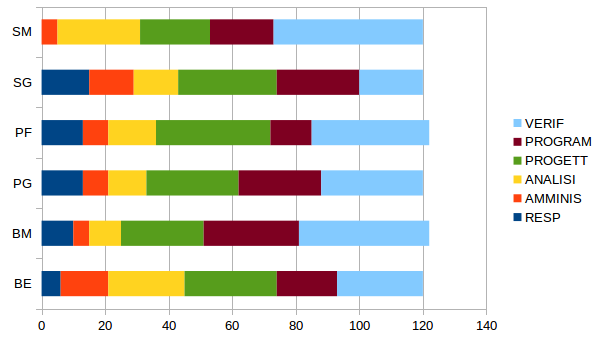
\includegraphics[scale=0.7]{Figures/OreComponenteRiepilogo.png}
				\caption{Riepilogo: ore per componente.}\label{fig:15}
			\end{figure}
			\begin{figure}[H]
				\centering
				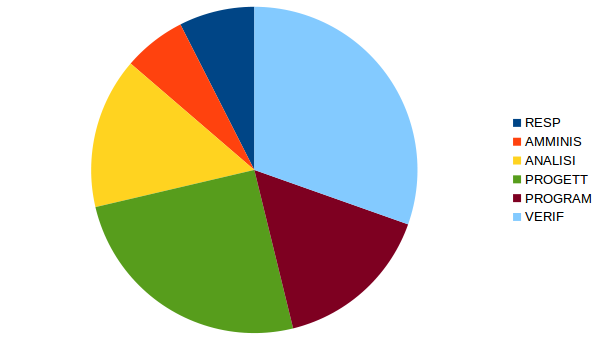
\includegraphics[scale=0.7]{Figures/OreRuoloRiepilogo.png}
				\caption{Riepilogo: ore per ruolo.}\label{fig:5}
			\end{figure}
			
		\subsubsection{Prospetto economico}
			\begin{table}[H]
				\center
				\begin{tabular}{|c|c|c|}
					\noalign{\hrule height 1.5pt}
					\textbf{Ruolo} & \textbf{Ore} & \textbf{Costo(\euro)}     \\
					\hline
					Responsabile  & 37 & 1110 \\ 
					\hline
					Amministratore  & 48  & 960 \\
					\hline
					Analista  & 108  & 2160 \\ 
					\hline
					Progettista  & 148 & 3256\\
					\hline
					Programmatore  & 98  & 1470\\
					\hline
					Verificatore  & 191 & 2865\\
					\hline
					\textbf{Totale}  & \textbf{630} & \textbf{11821}\\
					\noalign{\hrule height 1.5pt}
			\end{tabular}
			\caption{Riepilogo prospetto economico.  \label{tab:table_label}}
		\end{table}
		
\end{document}
